\chapter{Interval filament graphs}

\begin{defn}
	Given a half-plane $\pi$ with a border-line $l$, an \textbf{interval filament} in $\pi$ is a simple curve with
	endpoints on $l$, its interior lying in $\pi$ and within the stripe determined by lines perpendicular to $l$ and
	passing through the endpoints of the curve. The class of \textbf{interval filament graphs} is $\text{IFA} = \mathcal{IG}\{\text{interval filaments in a half-plane}\}$.
\end{defn}

\begin{figure}[!ht]\centering
	\begin{tikzpicture}
		\draw[color = gray] (2,0) -- (10,0);
		\node at (3,.3) {$l$};
		\draw[color=black, thick] (5,.01) edge (10,.01);
		\draw[dotted] (5,0) edge (5, 5);
		\draw[dotted] (10,0) edge (10,5);
		
		\draw[color=Red, thick] (5, .01) .. controls (10,5) and (4,3) .. (7, 4);
		\draw[color=Red, thick] (7, 4) .. controls (11,1) and (1,1) .. (10, .01);
		
		\fill[color=Red] (7,4) circle[radius=.35pt];
	\end{tikzpicture}
	\caption{An illustration to the definition. The name “interval-filament” comes from the fact that the curve “lives above” the interval that is determined by the endpoints of the filament on the boundary line $l$.}
\end{figure}

\begin{comm}
	If the base intervals of two interval-filaments overlap (i.e., they are not disjoint, but none of them is a subinterval of the other one), the filaments necessarily cross each other and the corresponding vertices in the intersection graph are adjacent (cf. the blue and red filaments in Fig. \ref{filaments}). On the other hand, if one of the base intervals is included in the other one, their filaments may or may not be disjoint (cf. the blue and yellow filaments for the disjoint case, and the red and green filaments for the non-disjoint one, both in Fig. \ref{filaments}).
\end{comm}

\begin{figure}[!ht]\centering
	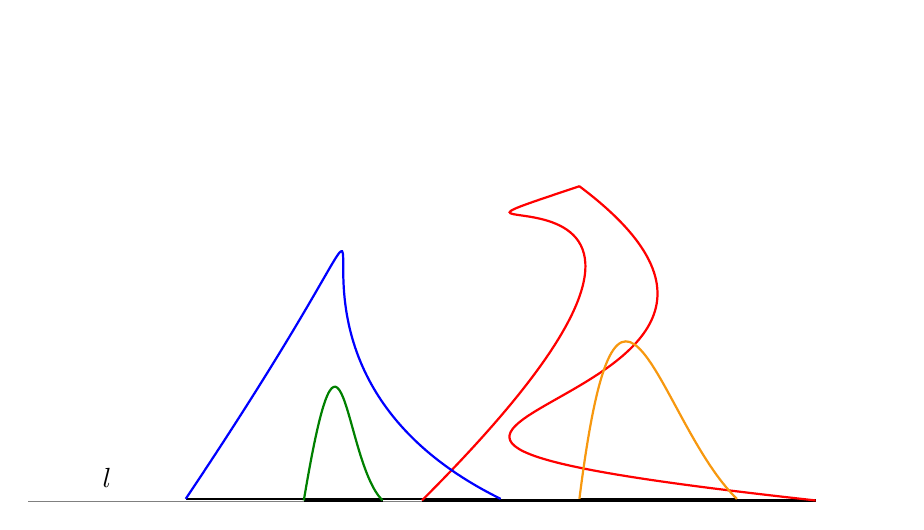
\begin{tikzpicture}
		\draw[color = gray] (0,0) -- (10,0);
		\node at (1,.3) {$l$};
		
		\draw[color=black, thick] (5,.01) edge (10,.01);
		\draw[color=black, thick] (7,.03) edge (9,.03);
		\draw[color=black, thick] (2,.03) edge (6,.03);
		\draw[color=black, thick] (3.5,.01) edge (4.5,.01);
		
		\draw[color=Red, thick] (5, .01) .. controls (10,5) and (4,3) .. (7, 4);
		\draw[color=Red, thick] (7, 4) .. controls (11,1) and (1,1) .. (10, .01);
		\fill[color=Red] (7,4) circle[radius=.35pt];
		
		\draw[color=Green, thick] (3.5, .01) .. controls (4,3) and (4,.5) .. (4.5, .01);
		\draw[color=Blue, thick] (2, .03) .. controls (6,6) and (2,2) .. (6, .03);
		\draw[color=YellowOrange, thick] (7, .03) .. controls (7.5,4) and (8,1) .. (9, .03);
	\end{tikzpicture}
	\caption{An illustration to the possible relative positions of interval-filaments.}
	\label{filaments}
\end{figure}